\documentclass[11pt]{amsart}
\usepackage{amsmath,amssymb,amsthm}
\usepackage{graphicx}
\usepackage{booktabs}
\usepackage[margin=1in]{geometry}
\usepackage{xr}
\externaldocument[M-]{main}
\usepackage{hyperref}

\newtheorem{theorem}{Theorem}[section]
\newtheorem{proposition}[theorem]{Proposition}
\newtheorem{lemma}[theorem]{Lemma}
\newtheorem{corollary}[theorem]{Corollary}
\theoremstyle{definition}
\newtheorem{definition}[theorem]{Definition}
\theoremstyle{remark}
\newtheorem{remark}[theorem]{Remark}

\newcommand{\ve}{\varepsilon}
\newcommand{\R}{\mathbb{R}}
\newcommand{\Z}{\mathbb{Z}}
\newcommand{\Lop}{\mathcal{L}}

\renewcommand{\thesection}{S\arabic{section}}
\renewcommand{\thefigure}{S\arabic{figure}}
\renewcommand{\thetable}{S\arabic{table}}

\title[Supplementary material]{Supplementary material to\\ ``The high activation energy limit of an equidiffusional flame model: rate of convergence and a convergent front-following scheme''}

\author{Juli\'an Fern\'andez Bonder}
\date{\today}

\begin{document}
\maketitle

This document contains the numerical experiments on travelling waves that are summarized
in Section~\ref{M-sec:exp:tw} of the article: the discretization error of the scheme (S) on
meshes that follow the front and on meshes that do not move, and a comparison of the
cost of the method with that of other solvers at equal accuracy. Numbers of sections,
theorems and equations without the prefix S refer to the article. In all the experiments
$f(s)=(1-s)^+$, unless stated otherwise, the meshes are those of
Section~\ref{M-sec:meshes} with $h_f=\ve/16$ and $h_c=0.01$, and the exact speed $c_\ve$ of the
travelling wave is computed by shooting (Section~\ref{M-sec:tw}). The code and the scripts
that produce every figure and table are available at
\url{https://github.com/jfbonder/combustion}.

\section{Travelling waves: the discretization error}\label{S:tw}

We start from the exact travelling wave, $U^0_j=\Phi_\ve(x_j-x_0)$, as in
Section~\ref{M-an:sec:ale}, with $A=1$, and record
\[
E=\max_{t_n\le T}\max_j\big|U^n_j-\Phi_\ve(x^n_j-x_0-c_\ve t_n)\big| ,
\]
the error $s_n$ in the position of the front, the error $E_s$ with the shift $s_n$
removed (which measures the profile), and, for ALE, the accumulated mesh-velocity
error $\mathcal M_T=\Delta t\sum_n|v_n-c_\ve|$ of Theorem~\ref{M-an:thm:ale}. Note that $E$ grows
linearly in time when the speed is wrong, while $E_s$ does not.

\emph{Inside the hypotheses of Theorem~\ref{M-an:thm:ale}.} On a uniform mesh with
$h=\ve^2/8$ and $\ve^2/16$, $\ve\in\{0.1,0.05\}$, translating rigidly with $v_n\equiv c_\ve$, we find
$E\le8\cdot10^{-6}$ at $T=3$ for $\Delta t=0.1$ and $\Delta t=0.01$: the error does not depend on the
time step, and the bound, with $\rho_hT=0.19$--$0.38$, is far from sharp. To test the
second alternative of the theorem we repeat the experiment with the rate
$f(s)=3\big((1-s)^+\big)^2$, which is of class $C^{1,1}(\R)$, and $h=\ve^{3/2}/k$, so that
$\rho_h=h^2/\ve^3=k^{-2}$. For $\ve=0.1$ and $k=2,4,8$ we find $E=7.7\cdot10^{-5}$,
$1.3\cdot10^{-5}$ and $4.1\cdot10^{-6}$ with $\Delta t=0.1$, and $8.8\cdot10^{-5}$, $1.8\cdot10^{-5}$ and
$5.8\cdot10^{-6}$ with $\Delta t=0.01$; for $\ve=0.05$ and $k=2,4$, $2.5\cdot10^{-5}$ and $3.9\cdot10^{-6}$
with $\Delta t=0.1$. The error is roughly proportional to $\rho_h$ (for $\ve=0.1$ it decreases by factors $5.7$
and $3.3$ when $\rho_h$ is divided by four), until it reaches the
accuracy of the reference profile (about $10^{-6}$), and a factor of ten in the time step
changes it by less than a factor $1.6$; the constant of the bound is again far from
sharp.

\emph{ALE with implicit velocity.} From now on $h_f=\ve/16$ and the mesh velocity is
computed. Figure~\ref{fig:D1} shows $E$ and $E_s$ for $\Delta t$ from $0.0025$ to $0.1$ and
$\ve\in\{0.01,0.003,0.001\}$, that is, $\Delta t/\ve$ up to $100$ and $\Delta t/\ve^2$ up to $10^5$. For
$w_0=0$ and $T=8$ we find $E=4.4$--$4.8\cdot10^{-4}$ and $E_s=4.3$--$4.4\cdot10^{-5}$ for all of
them ($E_s=6$--$7\cdot10^{-5}$ for $\Delta t=0.1$): no dependence on $\Delta t$ or on $\ve$. The same
values are found for $\ve=0.1$ and $\ve=0.05$ ($E=4.2$--$4.4\cdot10^{-4}$,
$E_s=4.1$--$4.3\cdot10^{-5}$), the range of realistic Zeldovich numbers. As
explained in Section~\ref{M-an:sec:impl}, $\mathcal M_T$ coincides with the error in the position of the
front, $7.7$--$8.3\cdot10^{-4}$, and $E\approx\Phi'(0)\mathcal M_T$; the maximum of $|v_n-c_\ve|$, on the
contrary, is attained in the first steps and grows as $\Delta t\to0$ (from $2.7\cdot10^{-4}$ for
$\Delta t=0.1$ to $1.6\cdot10^{-3}$ for $\Delta t=0.0025$). For $w_0=1$ ($c_\ve\approx1.63$) the same
holds if the rigid zone is long enough ($\ell_0=4$: $E\approx2.5\cdot10^{-3}$ at $T=4$,
$E_s\approx9\cdot10^{-5}$); with the default $\ell_0=2$ a term of order $\Delta t$ remains ($0.01\,\Delta t$
in the speed, growing slowly as $\ve$ decreases), the effect of the non-rigid far field
(Section~\ref{M-an:sec:impl}).

\begin{figure}[ht]
\centering
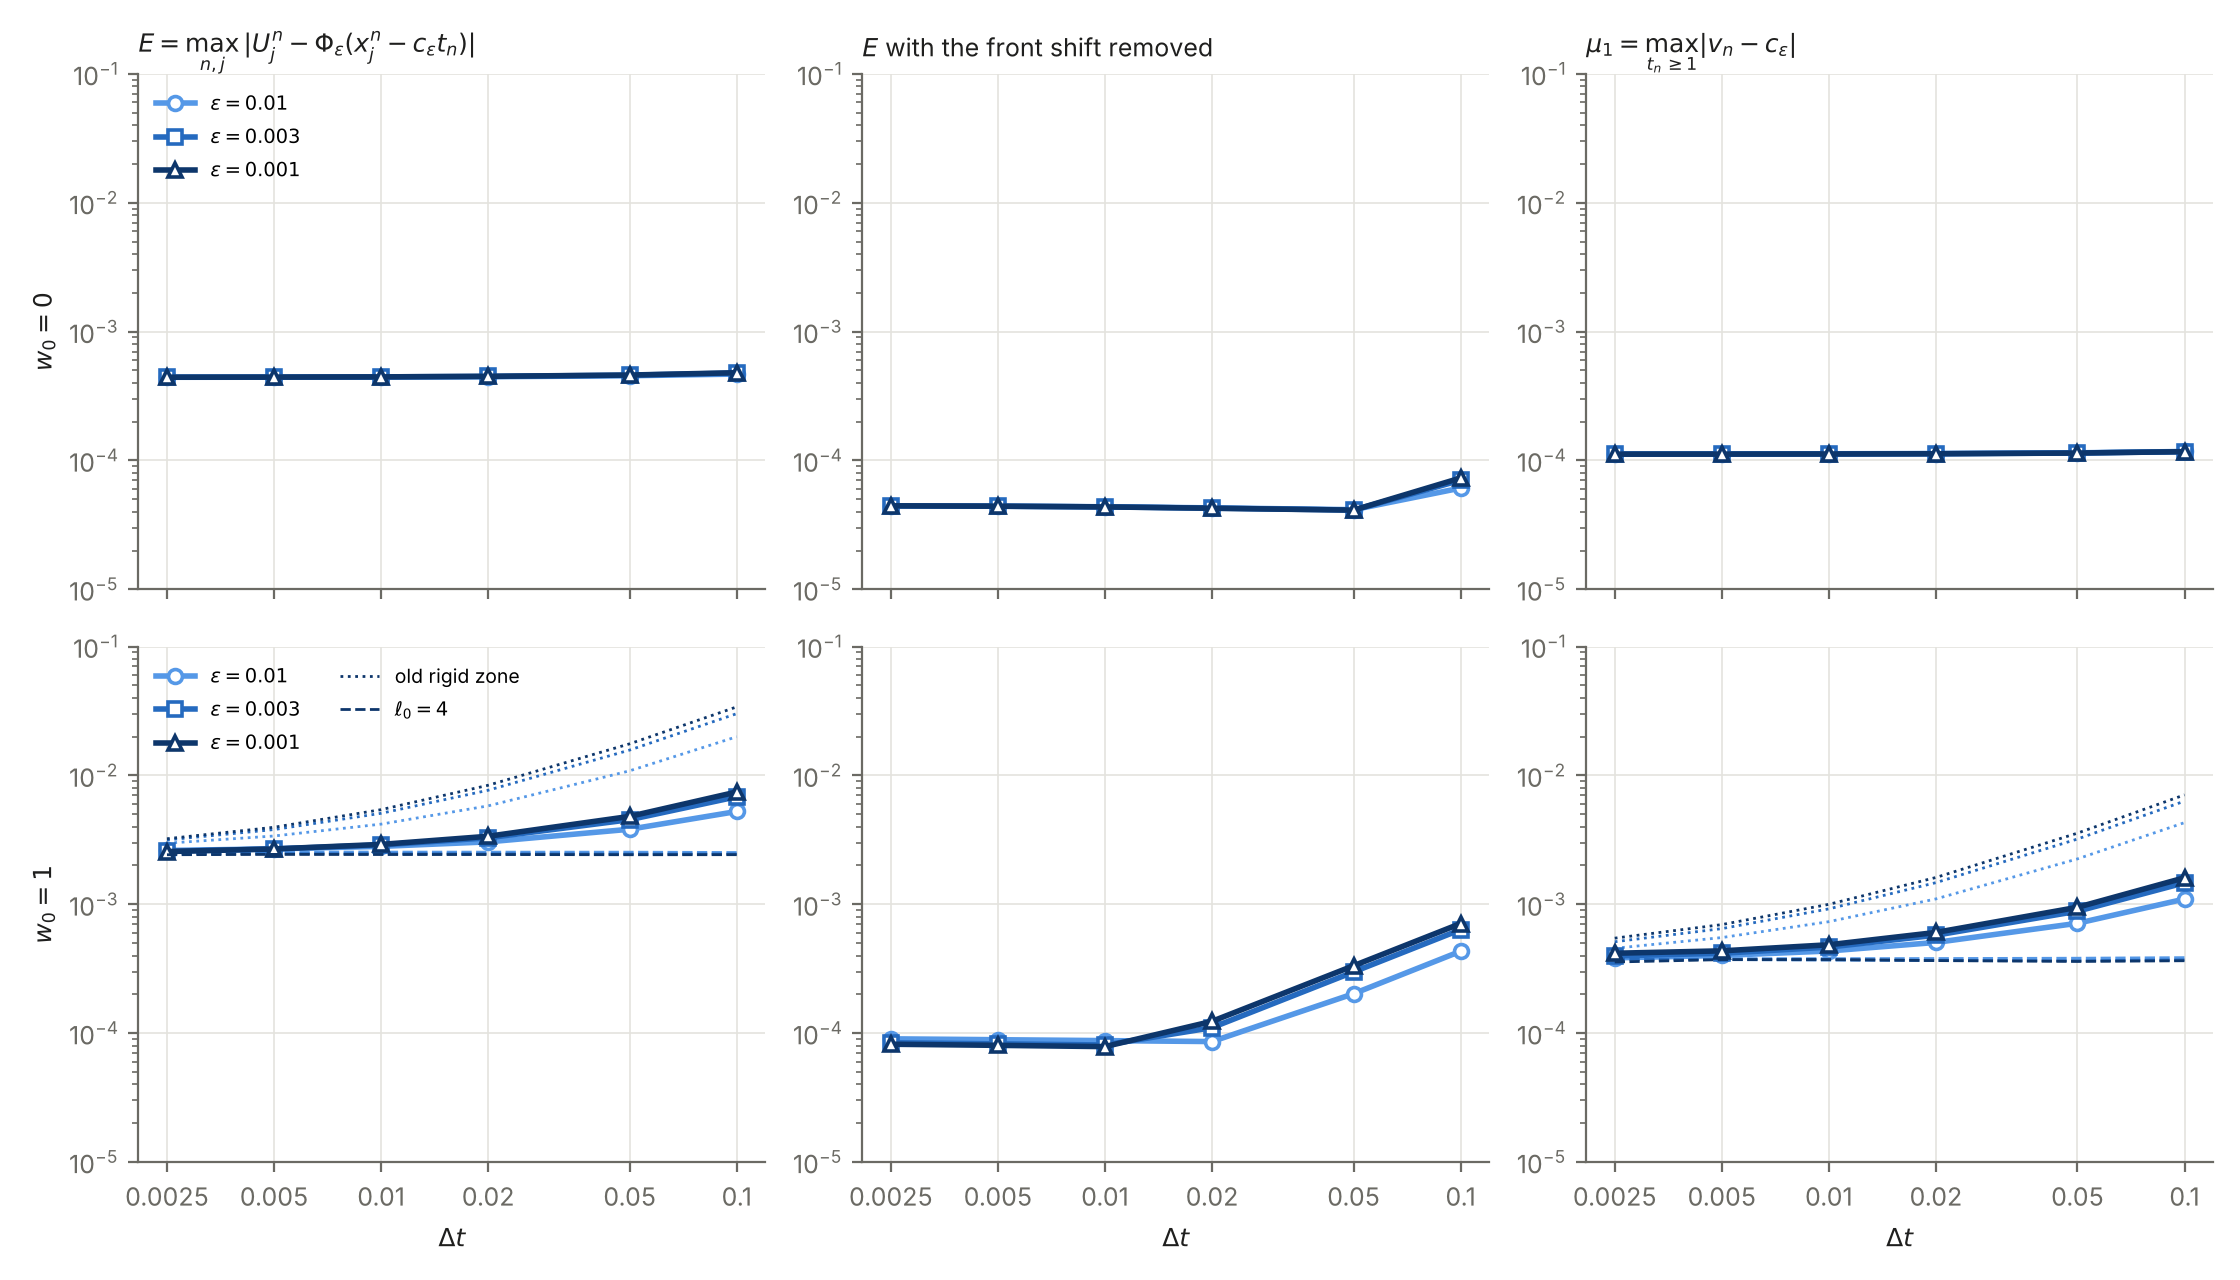
\includegraphics[width=0.9\textwidth]{../numerics/figures/paper/D1_ale_error_vs_dt.png}
\caption{ALE from $U^0=\Phi_\ve$: $E$, $E_s$, and $\max_{t_n\ge1}|v_n-c_\ve|$ against $\Delta t$,
for $\ve=0.01,0.003,0.001$. Top: $w_0=0$. Bottom: $w_0=1$ (solid: default $\ell_0$; dashed:
$\ell_0=4$; dotted: a shorter rigid zone).}\label{fig:D1}
\end{figure}

\emph{ALE: lattice pinning.} These values are for one position of the initial front
relative to the band lattice. With the implicit mesh velocity the front keeps its
position $\vartheta h_f$, $\vartheta\in[0,1)$, inside a band cell and, after a slow transient, it
travels with a speed $c_\ve+e(\vartheta)$ that depends on that position
(Figure~\ref{fig:D3}). The speed error $e(\vartheta)$ oscillates around a small offset
(about $10^{-5}$ for $w_0=0$ and $-6\cdot10^{-5}$ for $w_0=1$), with an amplitude proportional
to $(h_f/\ve)^2$: half of its range is $5.0\cdot10^{-4}$, $1.2\cdot10^{-4}$ and $3.1\cdot10^{-5}$ for
$h_f=\ve/8$, $\ve/16$ and $\ve/32$ ($w_0=0$), and $2.8\cdot10^{-3}$, $6.9\cdot10^{-4}$ and
$1.7\cdot10^{-4}$ for $w_0=1$, for $\ve=0.01$ and $\ve=0.001$ alike. Since the error in the
position grows linearly in time with slope $e(\vartheta)$, over $16$ values of $\vartheta$
($w_0=0$, $\ve=0.01$, $T=8$) $E$ ranges from $1.3\cdot10^{-5}$ to $9.5\cdot10^{-4}$, and $E_s$ from
$1.3\cdot10^{-5}$ to $9.6\cdot10^{-5}$. That the speed of a discrete travelling wave depends on its
position relative to the lattice is classical \cite{Keener1987}; for the freezing
method see \cite{Thummler2008SINUM}. Changing $\vartheta$ at every remeshing would not
average this error, because in the ALE version the mesh is rebuilt only a few times in a
run, and it would make the transfer inexact on the band. We have not looked for other
remedies; the error decreases like $(h_f/\ve)^2$.

\begin{figure}[ht]
\centering
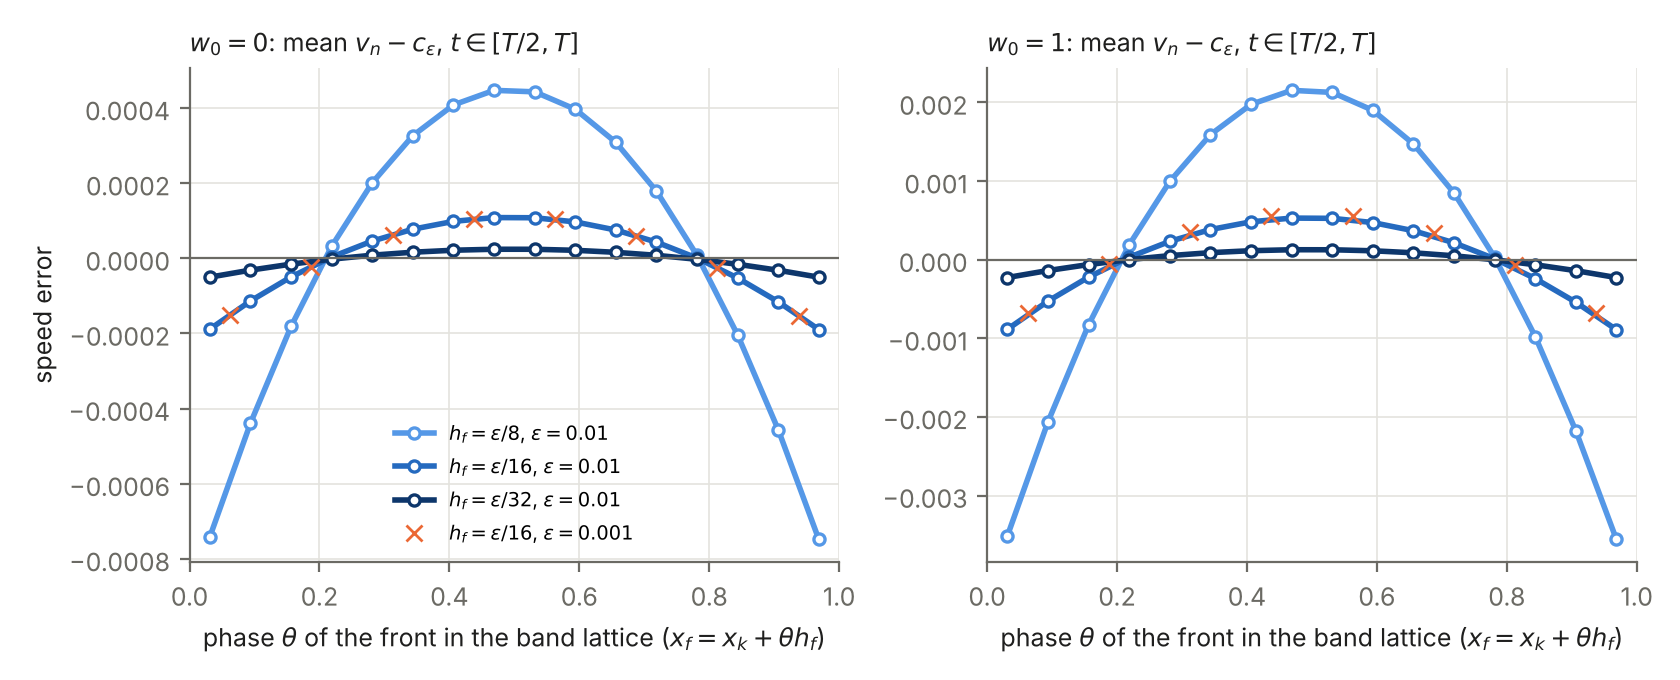
\includegraphics[width=0.85\textwidth]{../numerics/figures/paper/D3_phase_pinning.png}
\caption{ALE: speed error $e(\vartheta)$ against the position $\vartheta$ of the front in
its cell, measured after the transient (mean of $v_n-c_\ve$ on the last eighth of the run),
for $h_f/\ve=1/8,1/16,1/32$; lines: $\ve=0.01$, crosses: $\ve=0.001$.}\label{fig:D3}
\end{figure}

\emph{ALE: mesh sizes.} At a fixed $\vartheta$, and for $w_0=0$, the errors are of second
order in $h_f/\ve$ (a factor $3.9$--$4.3$ per halving, from $h_f=\ve/2$ to $\ve/32$) and the
values for different $\ve$ agree to one or two digits (Figure~\ref{fig:D2}); together with
Figure~\ref{fig:D3}, this is the scaling $(h_f/\ve)^2$ discussed in
Section~\ref{M-an:sec:impl}, not the $h_f/\ve$ of Theorem~\ref{M-cv:thm:main}. For $w_0=1$ the
last halving gives only a factor $1.4$--$3$, because the contribution of the coarse mesh,
roughly $O(h_c^2)$, takes over; for $w_0=0$ that contribution is at most $4\cdot10^{-5}$.

\begin{figure}[ht]
\centering
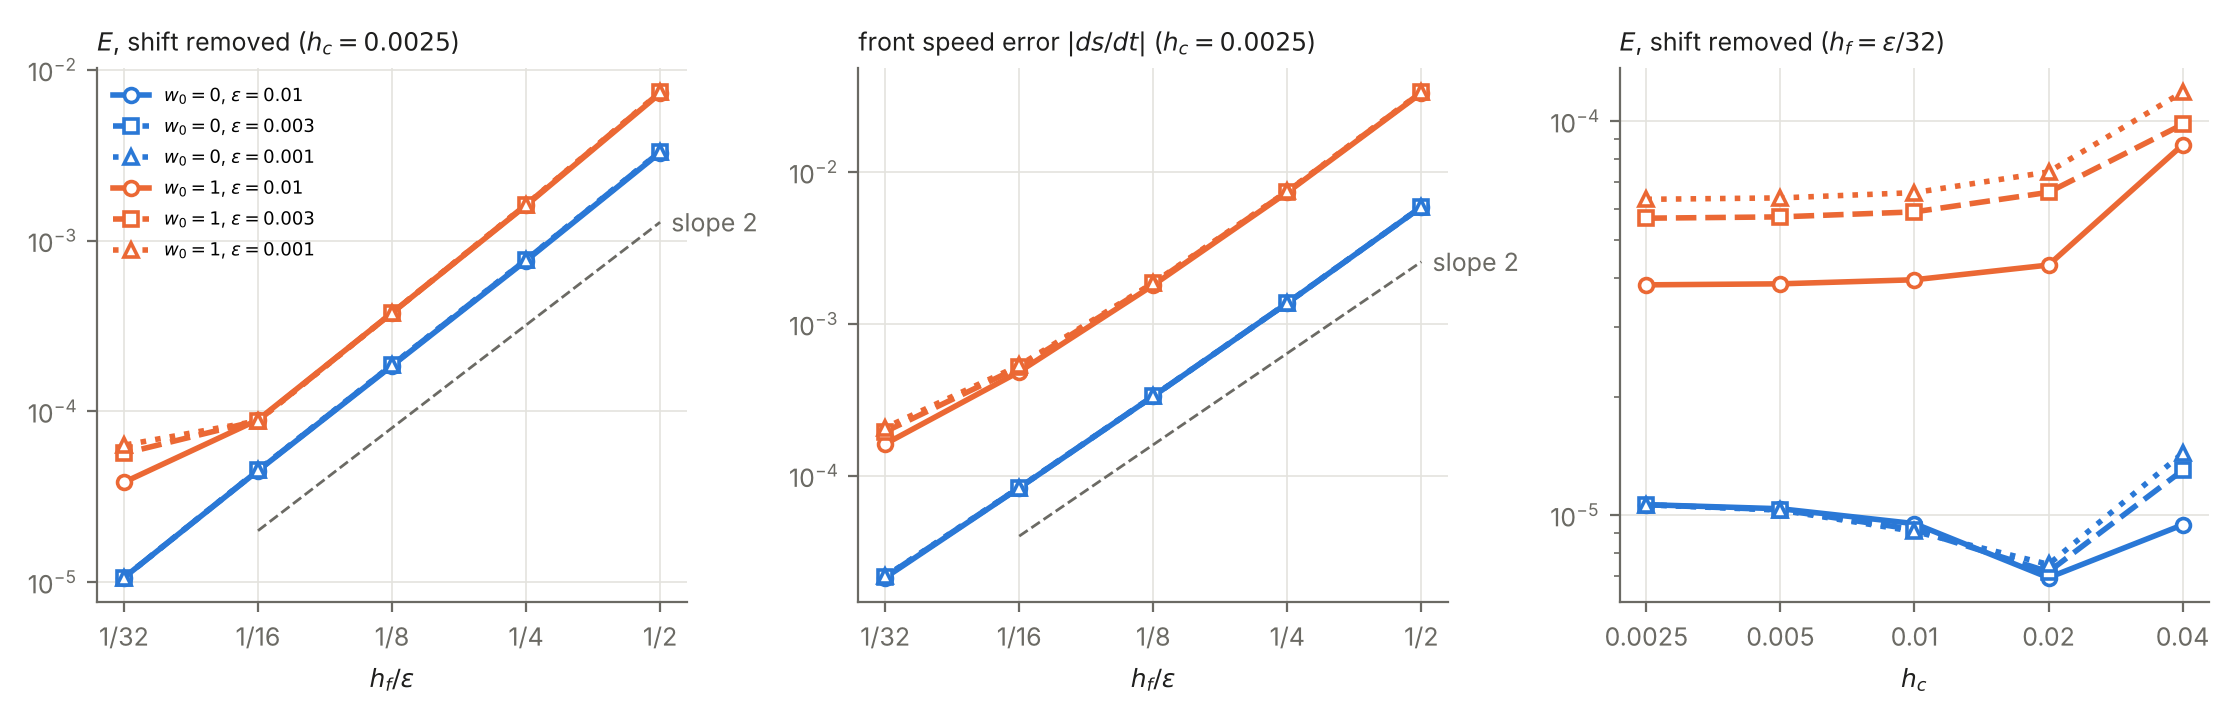
\includegraphics[width=\textwidth]{../numerics/figures/paper/D2_ale_error_vs_mesh.png}
\caption{ALE from $\Phi_\ve$, $\Delta t=0.01$, $\vartheta=0.37$, $T=8$ ($w_0=0$) or $4$ ($w_0=1$):
$E_s$ and speed error against $h_f/\ve$ (left, middle; $h_c=0.0025$) and against $h_c$
(right; $h_f=\ve/32$).}\label{fig:D2}
\end{figure}

\emph{The mesh drags the front.} On a rigid mesh translating with a prescribed
velocity $c_\ve+\delta v$, $\delta v=10^{-3}$, the speed of the front is
$c_\ve+\alpha\,\delta v$, where $\alpha$ is essentially a function of $\Delta t/\ve$: $\alpha=0.04$, $0.33$,
$0.84$ and $0.98$ for $\Delta t/\ve=0.03$, $1$, $10$ and $100$ ($w_0=0$). This is the factor
$\min\{1,\Delta t/\ve\}$ that multiplies $\mu$ in Theorem~\ref{M-cv:thm:main}, and the term $\mathcal M_n$ of
Theorem~\ref{M-an:thm:ale} is attained when $\Delta t\gg\ve$: for large time steps the front
locks to the mesh.

\emph{Fixed meshes: the lag.} With Eulerian (S) the front is slower than the exact one,
and the speed error is proportional to $\Delta t/\ve$, the order of
Theorem~\ref{M-cv:thm:main} for meshes that do not move. It settles slowly, on the time scale $4/c^2\approx12$ of the diffusive
relaxation ahead of the front (Figure~\ref{fig:D6}, left): measured on the window
$[54,60]$ it is between $-0.216$ and $-0.235$ times $\Delta t/\ve$ for the six cases of the
figure ($\Delta t/\ve$ from $0.0025$ to $0.08$), to be compared with the average
\eqref{M-an:eq:solv} of the truncation error, $-0.235\,\Delta t/\ve$. The differences are terms
of higher order in $\Delta t/\ve$ and a contribution of the coarse mesh, about $4\cdot10^{-5}$
in the speed when $h_c=\ve$, which disappears when $h_c$ is halved or the band is
widened. The same
slow relaxation is visible in the mesh velocity of the ALE scheme
(Figure~\ref{fig:D6}, right), which tends to $e(\vartheta)$.

\begin{figure}[ht]
\centering
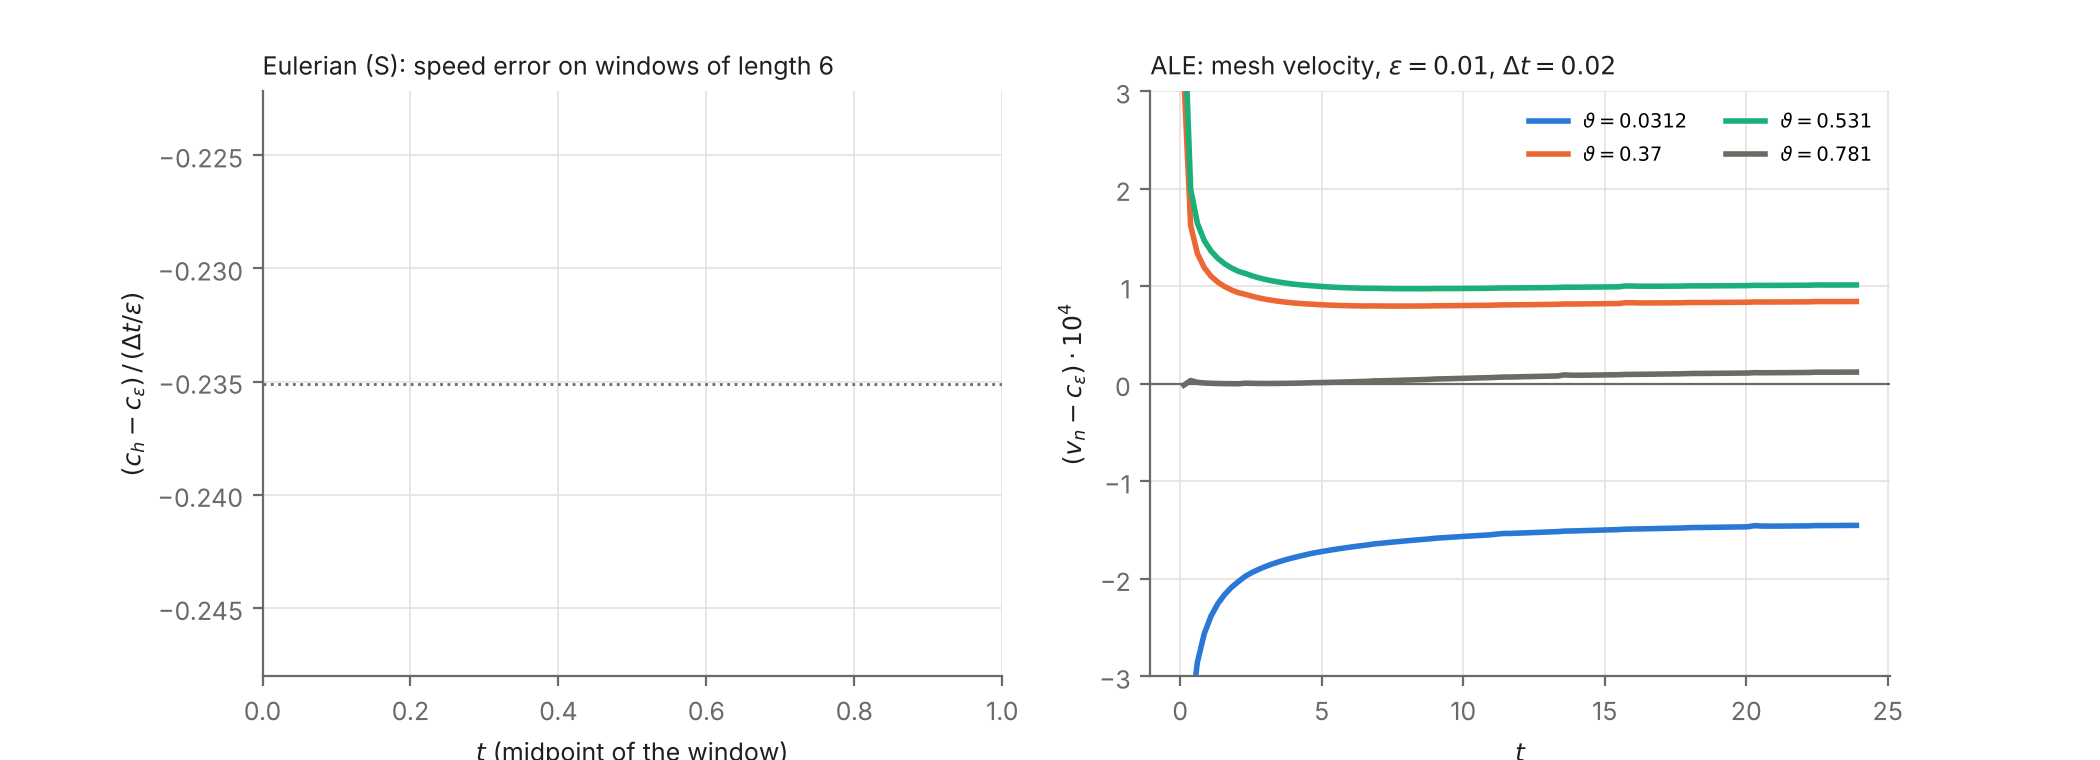
\includegraphics[width=\textwidth]{../numerics/figures/paper/D6_transients.png}
\caption{Left: Eulerian (S) from $\Phi_\ve$ ($w_0=0$): speed error on windows of length $6$,
divided by $\Delta t/\ve$; dotted: the value \eqref{M-an:eq:solv}. Right: ALE from $\Phi_\ve$
($\ve=0.01$, $\Delta t=0.02$): mesh velocity error $v_n-c_\ve$ for four positions $\vartheta$ of
the front in its cell.}\label{fig:D6}
\end{figure}

\section{Work and accuracy}\label{S:work}

For the planar travelling wave ($w_0=0$, $A=1$, started from $\Phi_\ve$, $0\le t\le4$) we
compare, at equal accuracy, the cost of five methods: ALE; the Eulerian version of (S),
on band meshes and, for $\ve=0.01$, on a uniform mesh of size $\ve/16$; the BDF solver of
Section~\ref{M-sec:eulerian}; and the same method of lines, on the same band meshes, with
the unknowns interleaved so that the Jacobian is banded, integrated with the variable
order solver LSODA and its banded linear algebra. Figure~\ref{fig:J1} shows the error in
the position of the front at $t=4$ against the running time, and Table~\ref{tab:work} gives
the number of steps and of linear solves, which do not depend on the implementation; the
times are those of our Python implementations on one core, and they are only indicative.

\begin{figure}[ht]
\centering
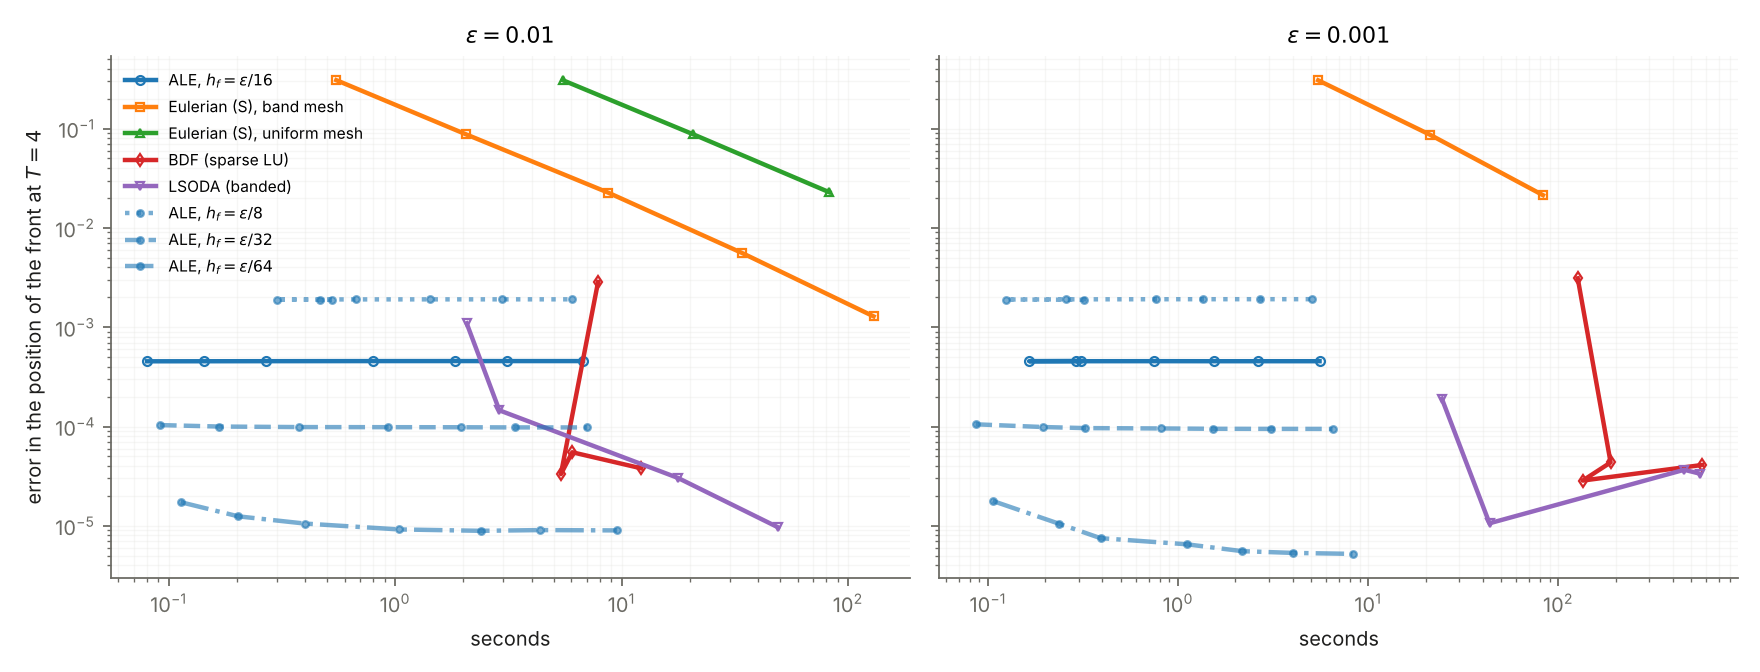
\includegraphics[width=\textwidth]{../numerics/figures/paper/J1_work_precision.png}
\caption{Planar travelling wave, $0\le t\le4$: error in the position of the front at the
final time against the running time. ALE with $\Delta t$ from $0.2$ to $0.0025$ and four band
mesh sizes; Eulerian (S) with $\Delta t=\ve/4,\dots,\ve/1024$; BDF and LSODA with relative
tolerances from $10^{-3}$ to $10^{-6}$.}\label{fig:J1}
\end{figure}

\begin{table}[ht]
\centering
\footnotesize
\setlength{\tabcolsep}{4pt}
\begin{tabular}{l ccc ccc}
\toprule
& \multicolumn{3}{c}{$\ve=0.01$} & \multicolumn{3}{c}{$\ve=0.001$}\\
method & error & steps & solves & error & steps & solves\\
\midrule
ALE, $\ve/16$, $\Delta t=0.1$  & $4.5\cdot10^{-4}$ & $40$ & $240$ & $4.6\cdot10^{-4}$ & $40$ & $240$\\
ALE, $\ve/32$, $\Delta t=0.1$  & $1.0\cdot10^{-4}$ & $40$ & $240$ & $9.9\cdot10^{-5}$ & $40$ & $240$\\
ALE, $\ve/64$, $\Delta t=0.01$ & $8.9\cdot10^{-6}$ & $400$ & $2400$ & $5.6\cdot10^{-6}$ & $400$ & $2400$\\
BDF, rtol $10^{-4}$                & $3.3\cdot10^{-5}$ & $727$ & $999$ & $4.4\cdot10^{-5}$ & $23397$ & $49297$\\
BDF, rtol $10^{-5}$                & $5.5\cdot10^{-5}$ & $907$ & $1174$ & $2.9\cdot10^{-5}$ & $23301$ & $31322$\\
LSODA, rtol $10^{-4}$              & $1.5\cdot10^{-4}$ & $2732$ & $651$ & $1.1\cdot10^{-5}$ & $45420$ & $13597$\\
LSODA, rtol $10^{-5}$              & $3.0\cdot10^{-5}$ & $17074$ & $5707$ & $3.7\cdot10^{-5}$ & $413042$ & $184098$\\
Eul.\ (S), $\Delta t=\ve/64$     & $2.3\cdot10^{-2}$ & $25600$ & $51200$ & $2.1\cdot10^{-2}$ & $256000$ & $512000$\\
Eul.\ (S), $\Delta t=\ve/1024$   & $1.3\cdot10^{-3}$ & $409600$ & $819200$ & & &\\
\bottomrule
\end{tabular}
\caption{Planar travelling wave, $0\le t\le4$: error in the position of the front at the
final time, number of time steps, and number of linear solves; for ALE the first entry
is $h_f$ (tridiagonal solves for
(S), sparse LU factorizations of the $2J\times2J$ Jacobian for BDF, banded Jacobian
evaluations and factorizations for LSODA). The meshes have between $3100$ and $6300$
nodes.}\label{tab:work}
\end{table}

For ALE the error is determined by the mesh of the band: $1.9\cdot10^{-3}$, $4.5\cdot10^{-4}$,
$1.0\cdot10^{-4}$ and about $10^{-5}$ for $h_f=\ve/8$, $\ve/16$, $\ve/32$ and $\ve/64$, for both values
of $\ve$ and for every time step between $0.0025$ and $0.2$. (This is the lattice pinning
error for the phase $\vartheta=0.37$ of these runs; for other phases it lies between much
smaller values and about twice this one, see Section~\ref{S:tw}.) Hence the largest
time step can be used, and the cost, $240$
tridiagonal solves, a few tenths of a second, does not depend on $\ve$. The two
method-of-lines solvers reach errors between $10^{-5}$ and $6\cdot10^{-5}$, which they do not
improve when the tolerance is reduced, because of the transfers between the band
meshes, which are rebuilt about $30$ times for $\ve=0.01$ and $300$ times for $\ve=0.001$. For
errors below $10^{-4}$ BDF needs $700$ to $900$ steps and $5$ to $6$ seconds for $\ve=0.01$, and
$2.3\cdot10^4$ steps and $130$ to $190$ seconds for $\ve=0.001$ (its number of steps grows like
$\ve^{-1.4}$); LSODA needs $1.7\cdot10^4$ steps and $18$ seconds, and $4.5\cdot10^4$ steps and
$43$ seconds. The banded solver is
faster per step than the sparse one, but the number of steps, not the linear algebra, is
what makes these methods expensive for small $\ve$. For the Eulerian version of (S) the
error is proportional to $\Delta t/\ve$, between $0.31$ and $0.36$ times $(\Delta t/\ve)\,T$ (the
coefficient $0.23$ of Section~\ref{S:tw} is reached only after the transient), on
band meshes and on the uniform mesh alike, and an error of $10^{-3}$ already requires
$\Delta t\approx\ve/1000$.

Two remarks limit the scope of this comparison. First, the travelling wave is the most
favourable case for ALE, because the solution is steady in the frame of the band and the
time step does not enter the error; for other data the error is of first order in
$\Delta t$ (Section~\ref{M-sec:exp:thm}), and the time step has to be chosen accordingly.
Second, we have not compared with moving mesh methods based on equidistribution
\cite{HuangRussell2011}, which are the natural alternative to a band that follows the
front.


\bibliographystyle{amsplain}
\bibliography{references}

\end{document}
